\newpage

\newgeometry{left=1.5in, right=1in, top=1in, bottom=1in}

\titleformat{\section}{\normalfont\bfseries}{\thesection}{1em}{}

%\setcounter{section}{1}

%\begin{appendices}
%    \chapter*{APPENDICES}

\begin{center}
	\MakeUppercase{\textbf{APPENDICES}}
\end{center}

%\newpage
%\clearpage
\addcontentsline{toc}{chapter}{\MakeUppercase{APPENDICES}}


\section*{Appendix 1: Log Targets} \label{app:log-targets}

    This subsection presents the log - target plots for the remaining spatio-temporal LGCP models.

    \begin{figure}[H]
        \begin{center}
            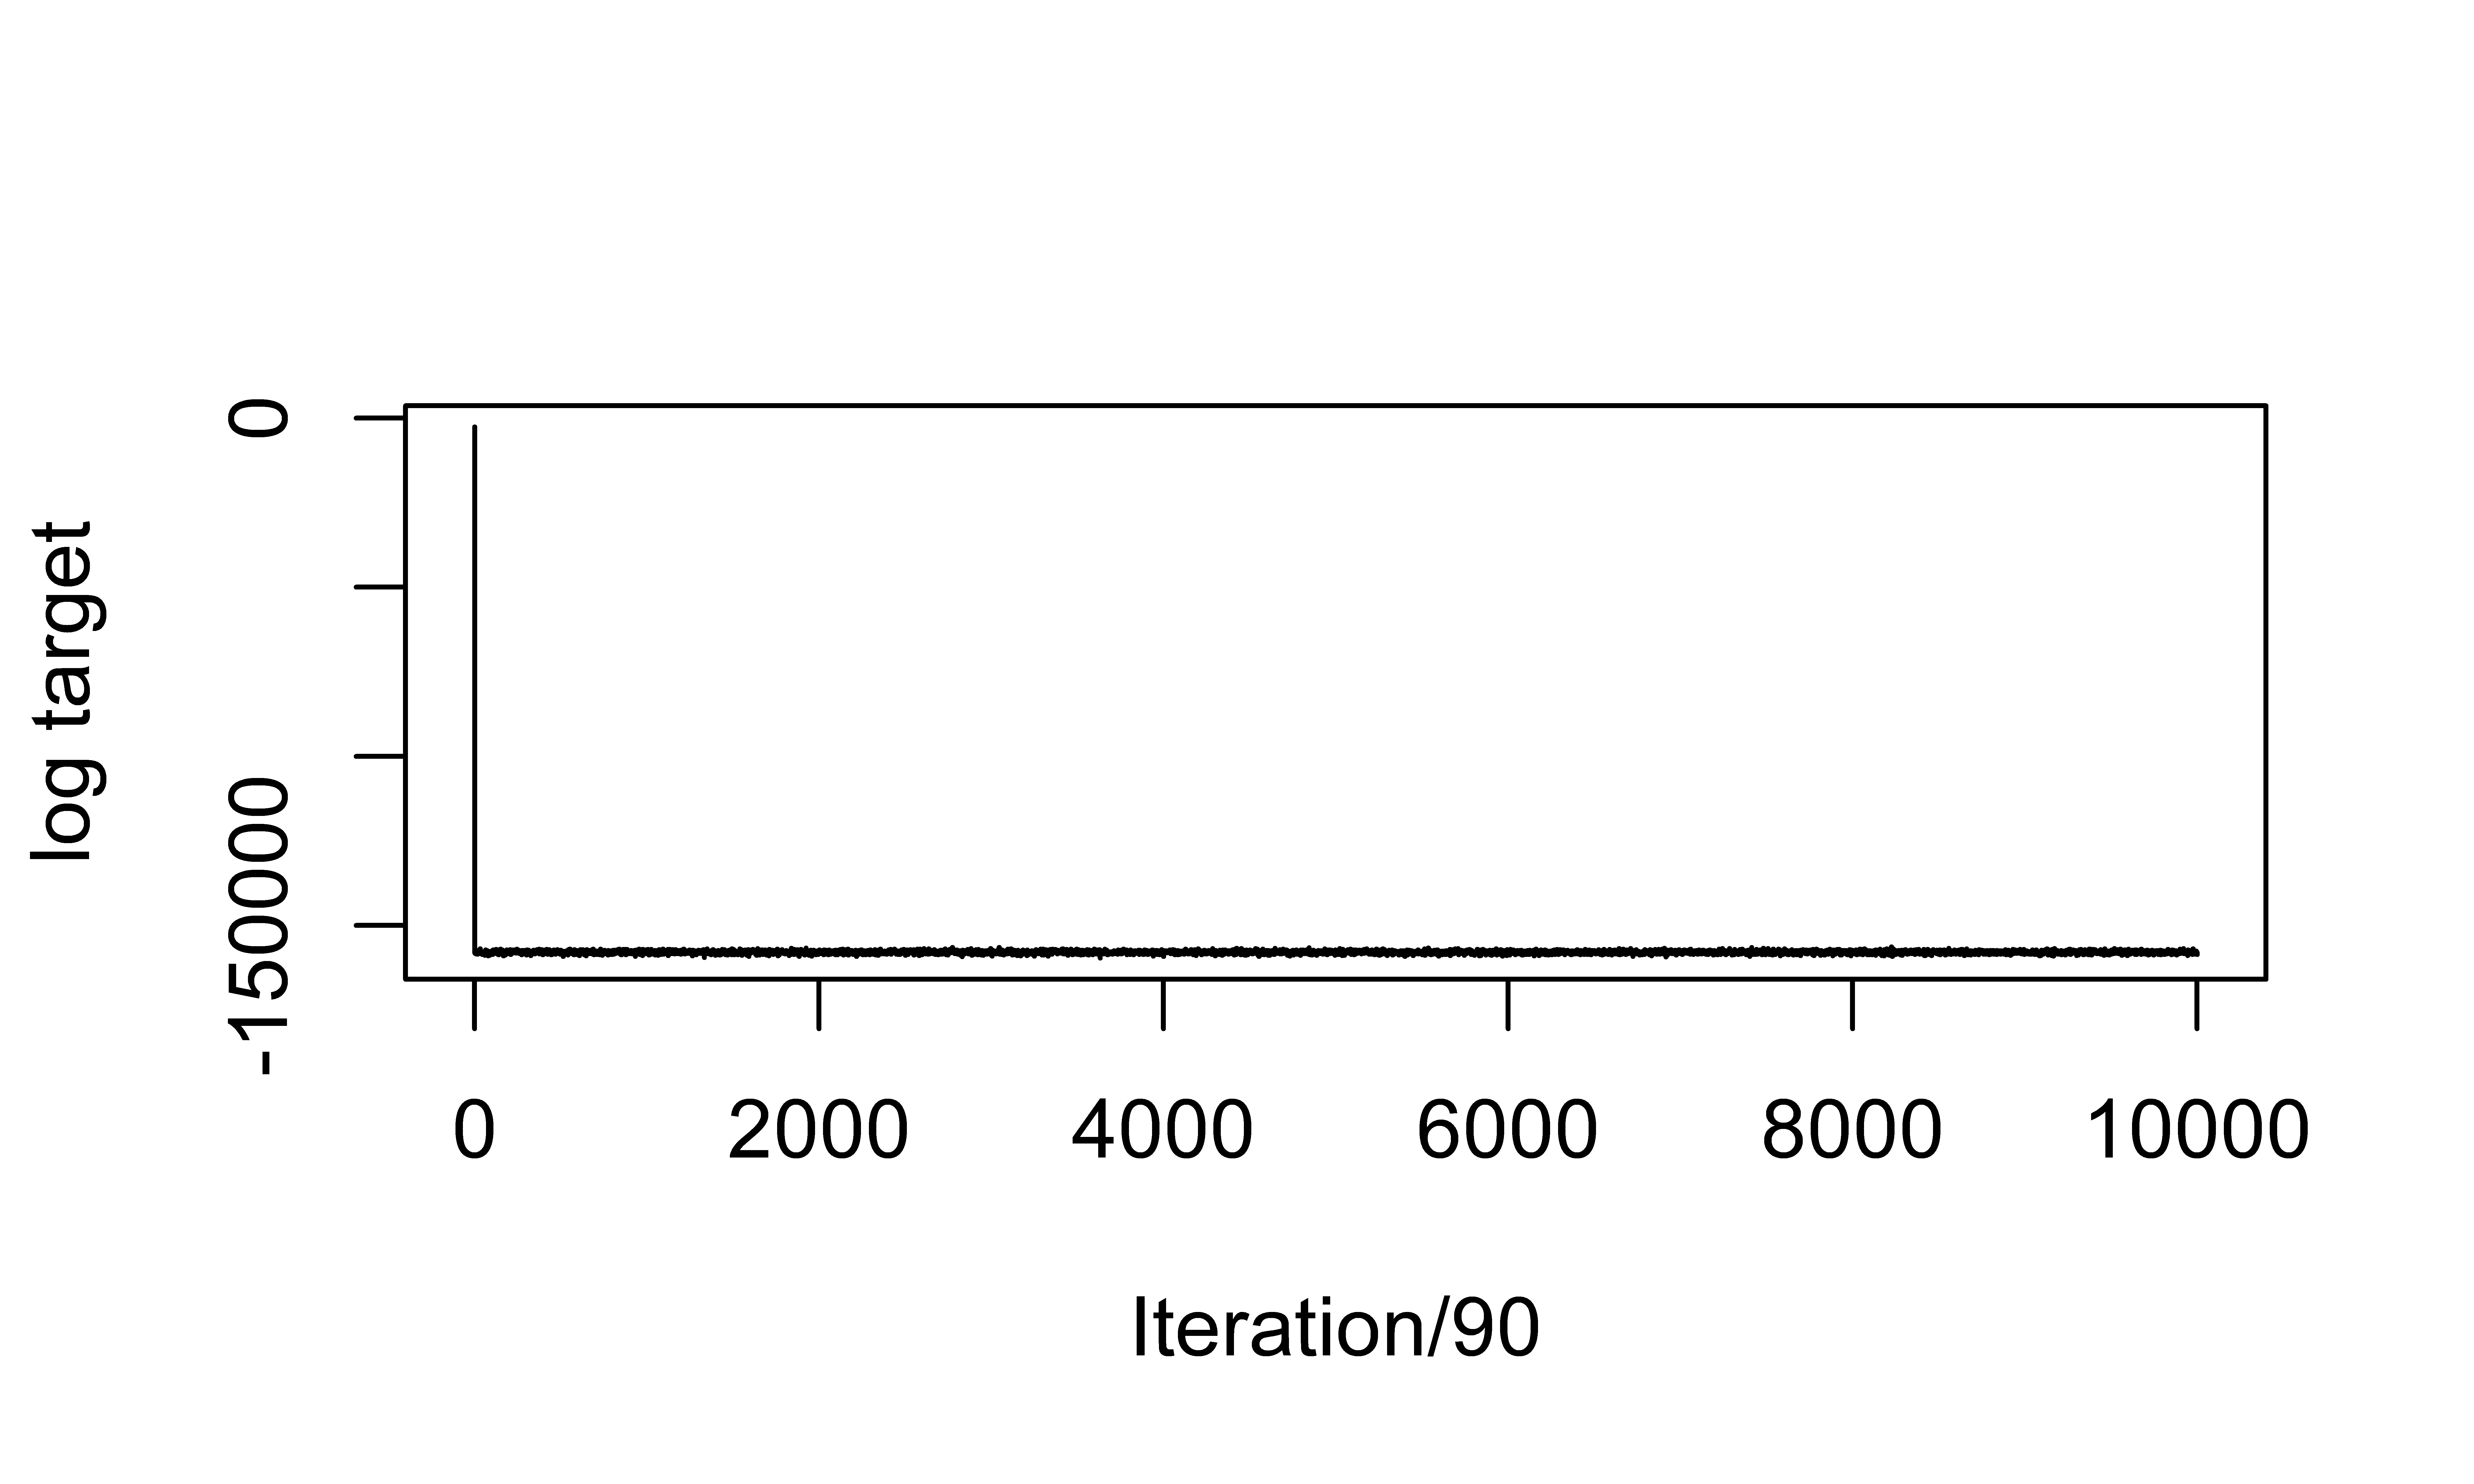
\includegraphics[scale=1]{Log Target Plot - ST - Major 0.png}
        \end{center}
        \FigureCaption{Log target plot for the spatio-temporal model for clade 0}
    \end{figure}

    \begin{figure}[H]
        \begin{center}
            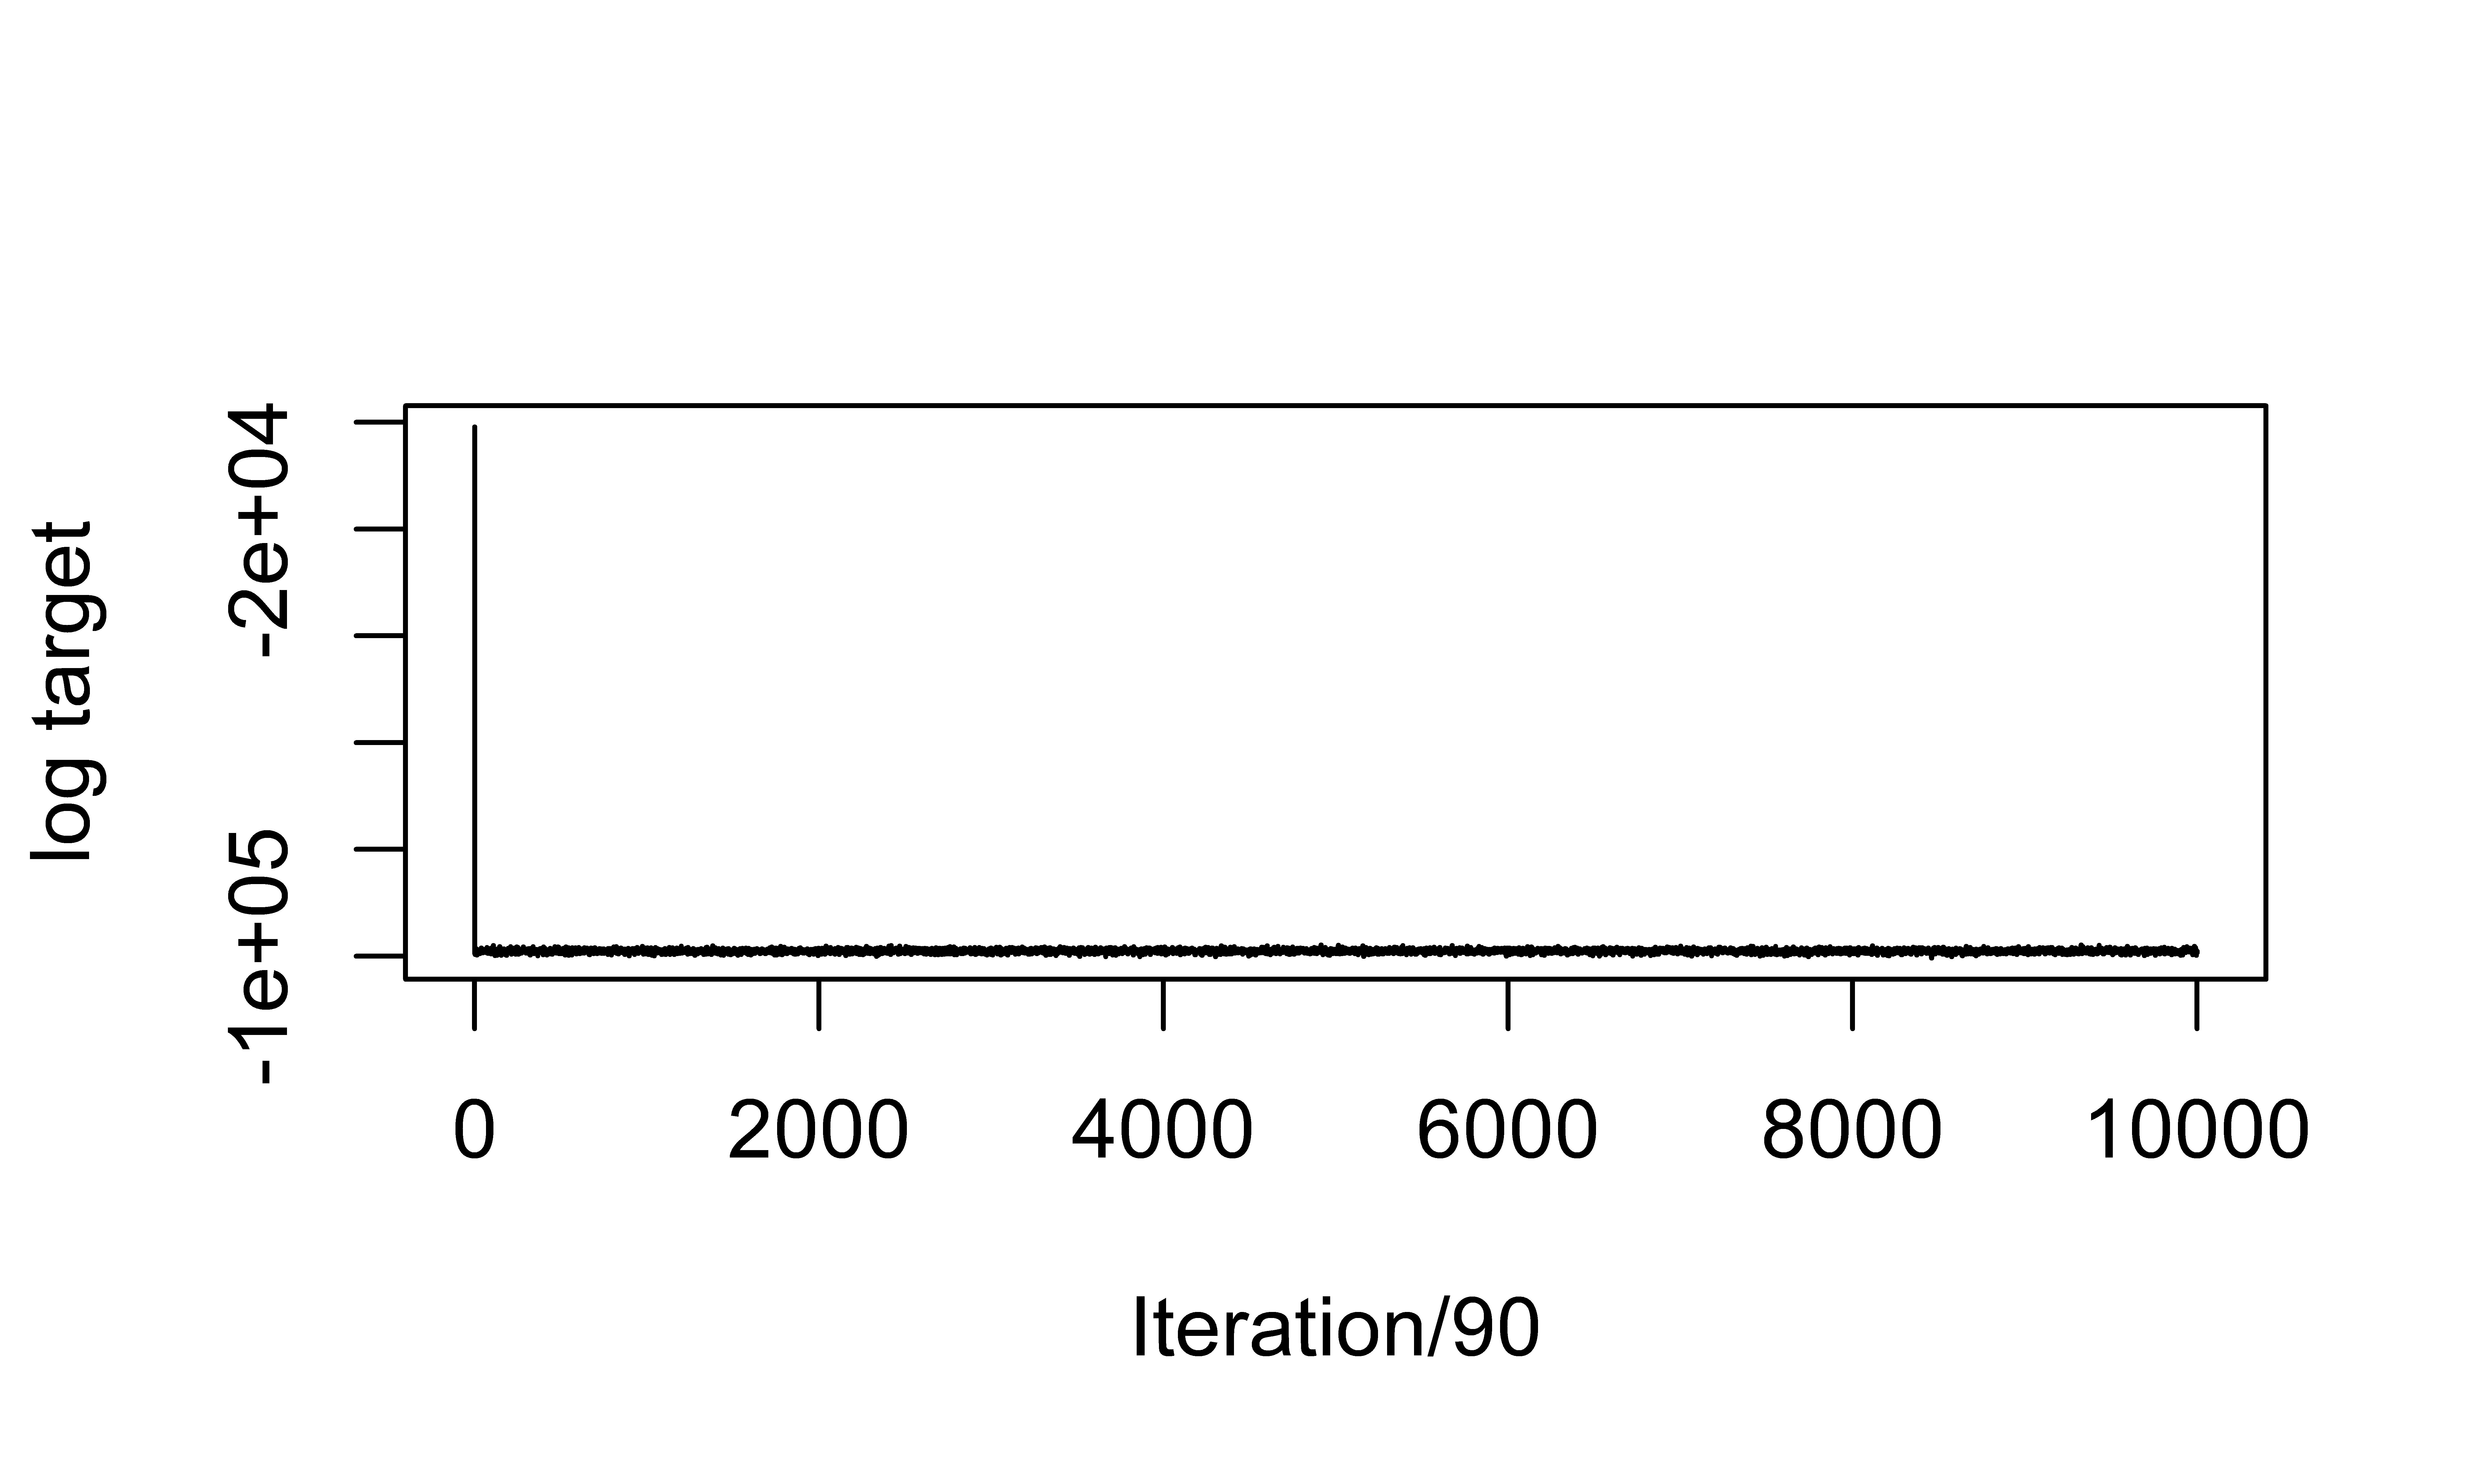
\includegraphics{Log Target Plot - ST - Major 2.png}
        \end{center}
        \FigureCaption{Log target plot for the spatio-temporal model for clade 2}
    \end{figure}

\restoregeometry

    \begin{figure}[H]
        \begin{center}
            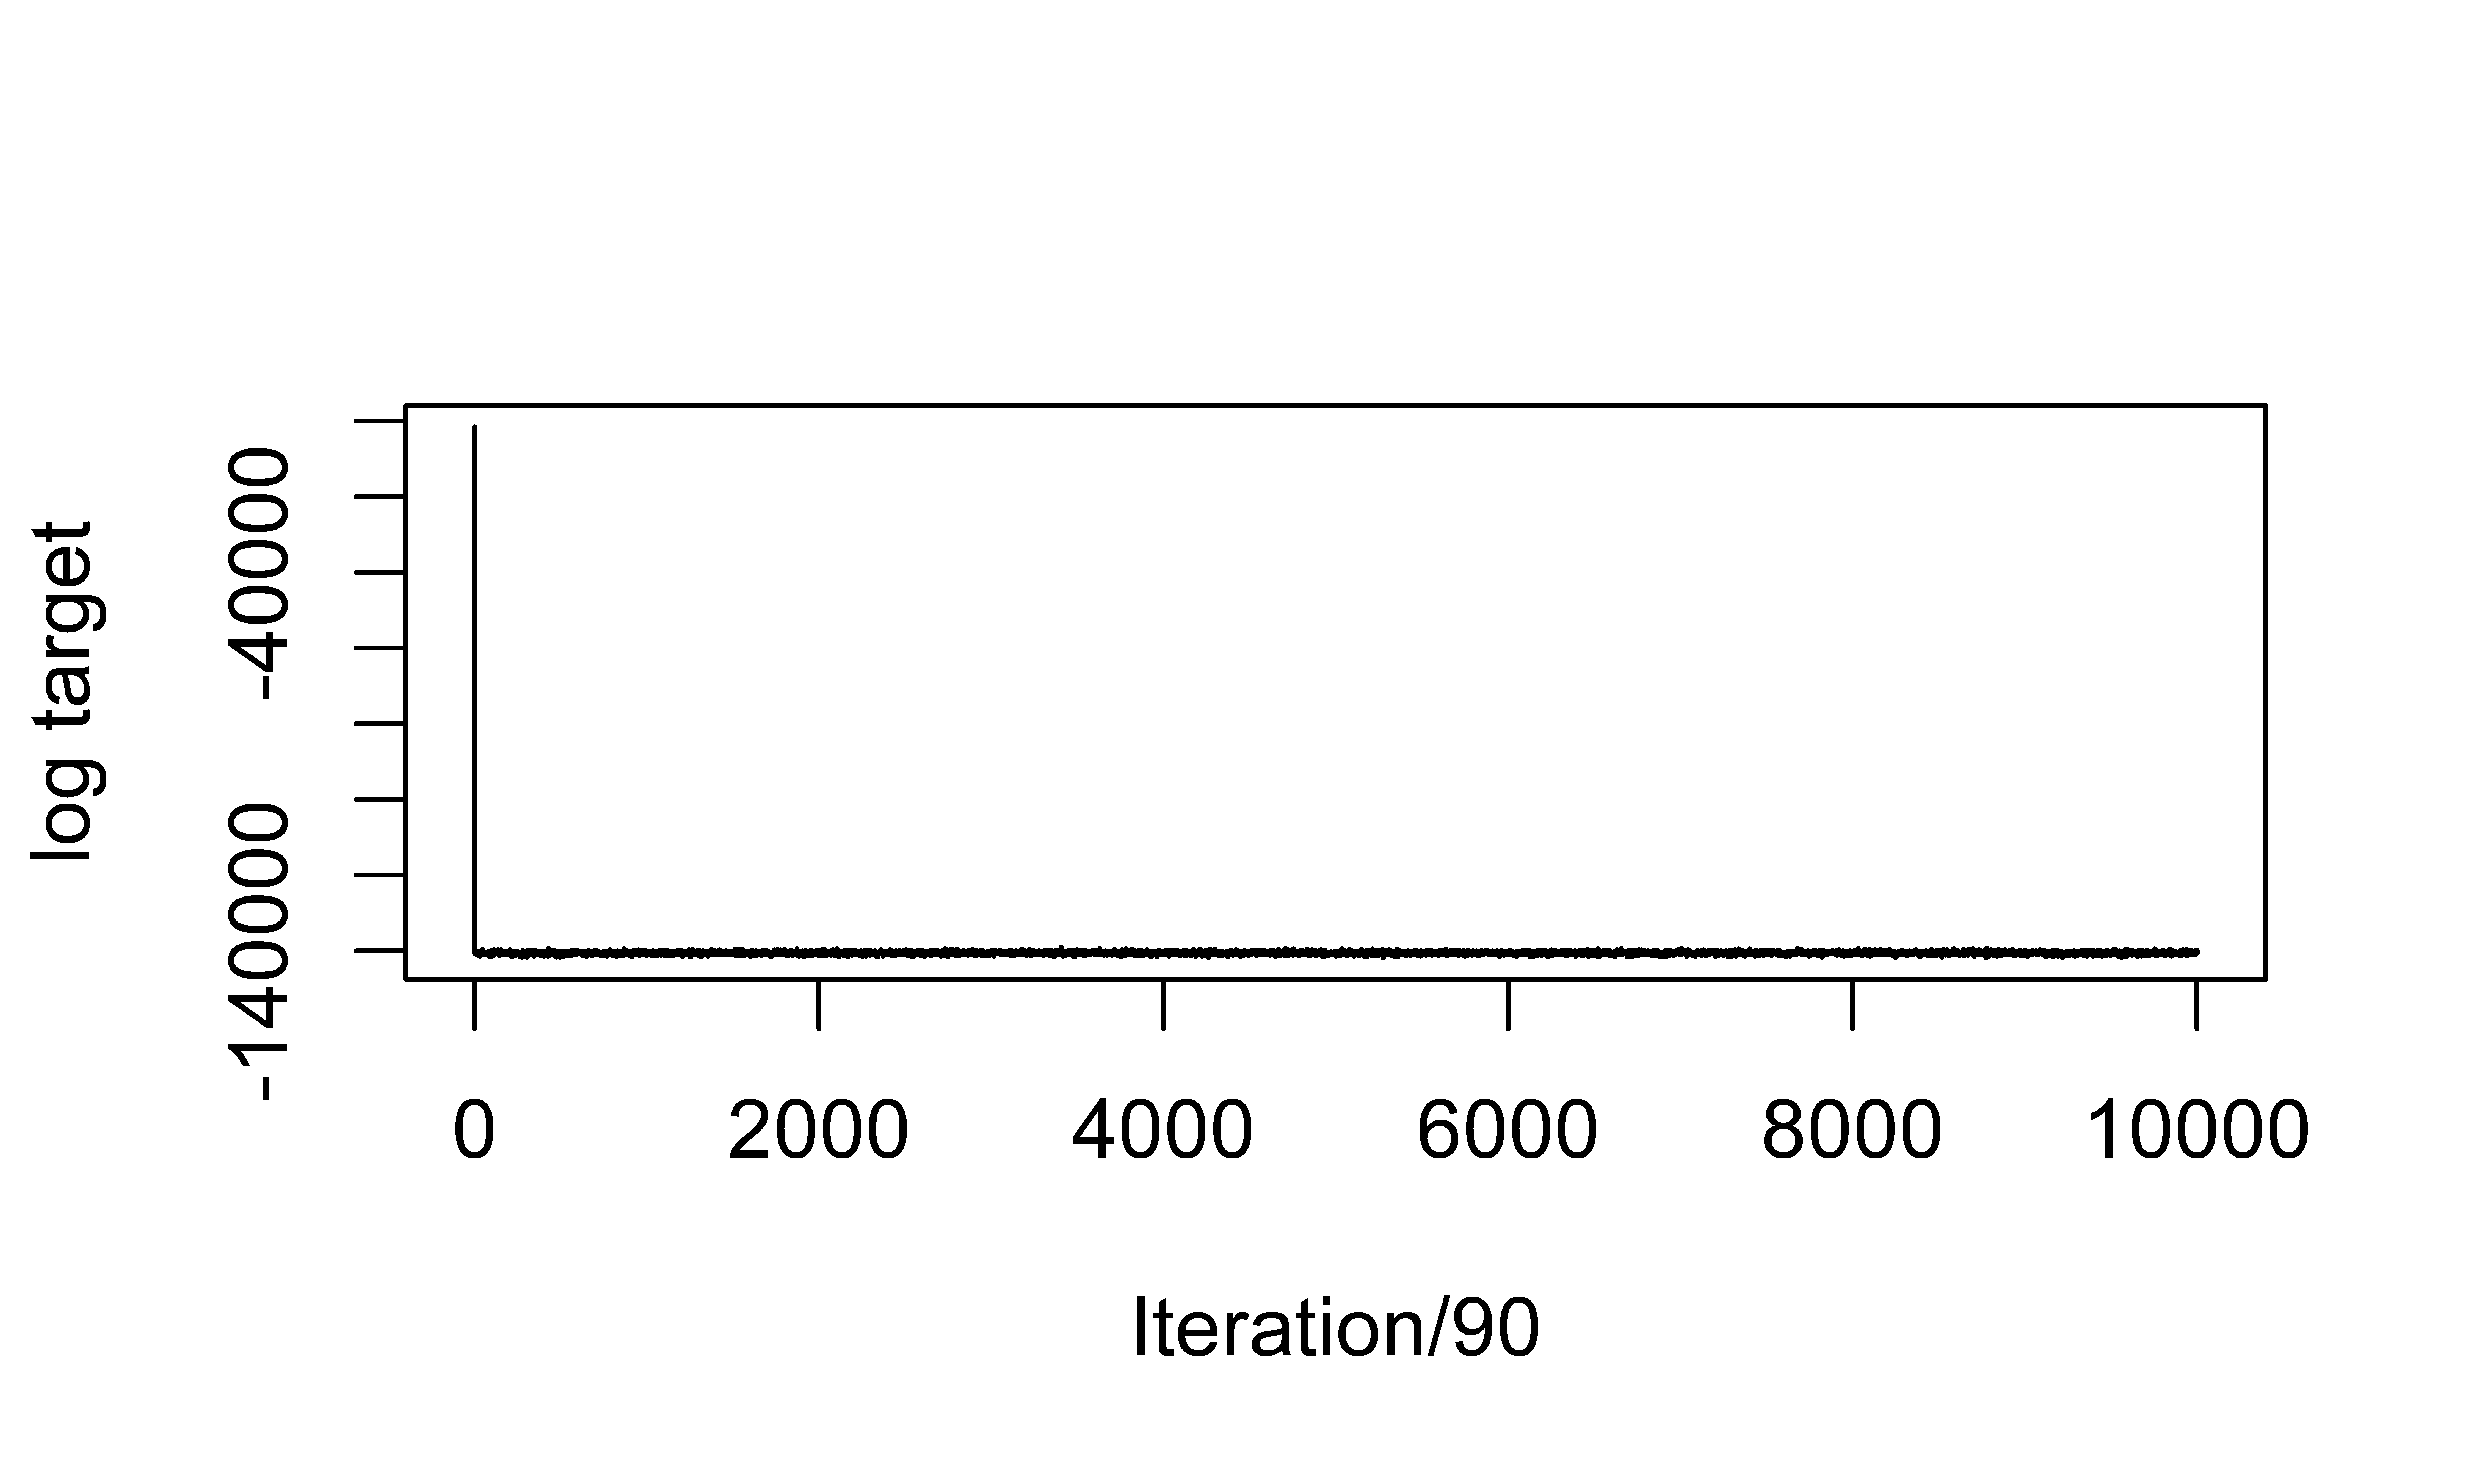
\includegraphics{Log Target Plot - ST - Major 13456.png}
        \end{center}
        \FigureCaption{Log target plot for the spatio-temporal model for the grouped clades}
    \end{figure}

    \newpage

\section*{Appendix 2: Traceplots} \label{app:trace-plots}

    This subsection presents the traceplots for the remaining spatio-temporal LGCP models.

    \begin{figure}[H]
        \begin{center}
            \includegraphics[width = \linewidth, height = 80mm]{Traceplots for Beta and Eta - Major 0.png}
        \end{center}
        \FigureCaption{Traceplots for Beta and Eta for clade 0 cases}
    \end{figure}

    \begin{figure}[h]
        \begin{center}
            \includegraphics[width = \linewidth, height = 80mm]{Traceplots for Beta and Eta - Major 2.png}
        \end{center}
        \FigureCaption{Traceplots for Beta and Eta for clade 2 cases}
    \end{figure}

    \begin{figure}[H]
        \begin{center}
            \includegraphics[width = \linewidth, height = 80mm]{Traceplots for Beta and Eta - Major 13456.png}
        \end{center}
        \FigureCaption{Traceplots for Beta and Eta for the grouped clades}
    \end{figure}

    \newpage


\section*{Appendix 3: Autocorrelation in the Latent Field} \label{app:latent-field}

    This subsection presents plots of the autocorrelations in the latent field for different lags for the remaining spatio-temporal LGCP models.

    \begin{figure}[H]
        \begin{center}
            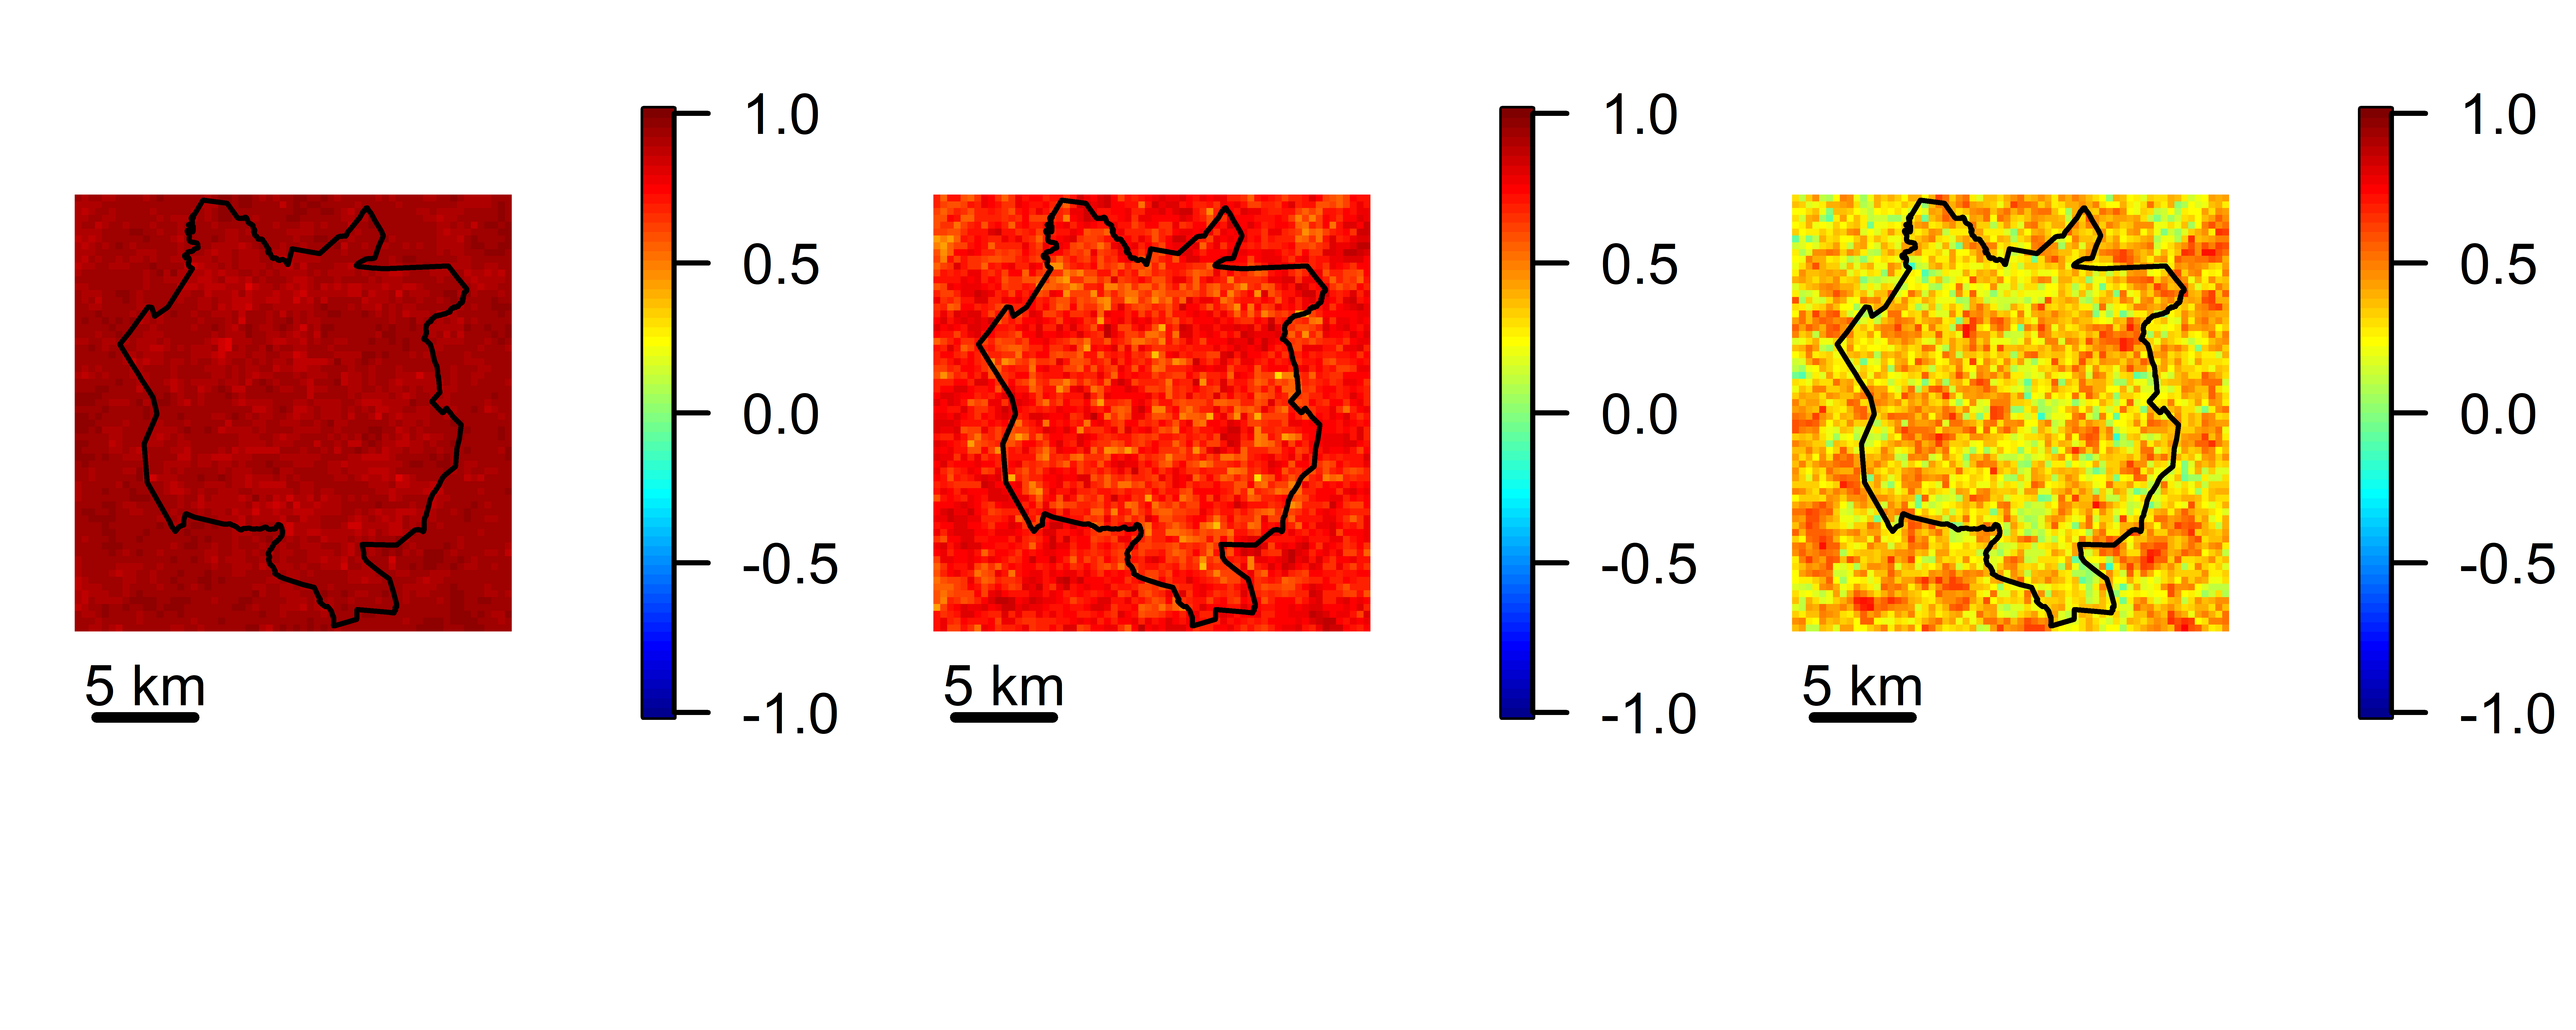
\includegraphics[width = \linewidth, height = 60mm]{Autocorrelations in the Latent Field - All Cases.png}
        \end{center}
        \FigureCaption{Left to right: autocorrelations in the Gaussian latent field at lag 1, lag 5 and lag 15 for spatio-temporal model with all cases}
    \end{figure}

    \begin{figure}[H]
        \begin{center}
            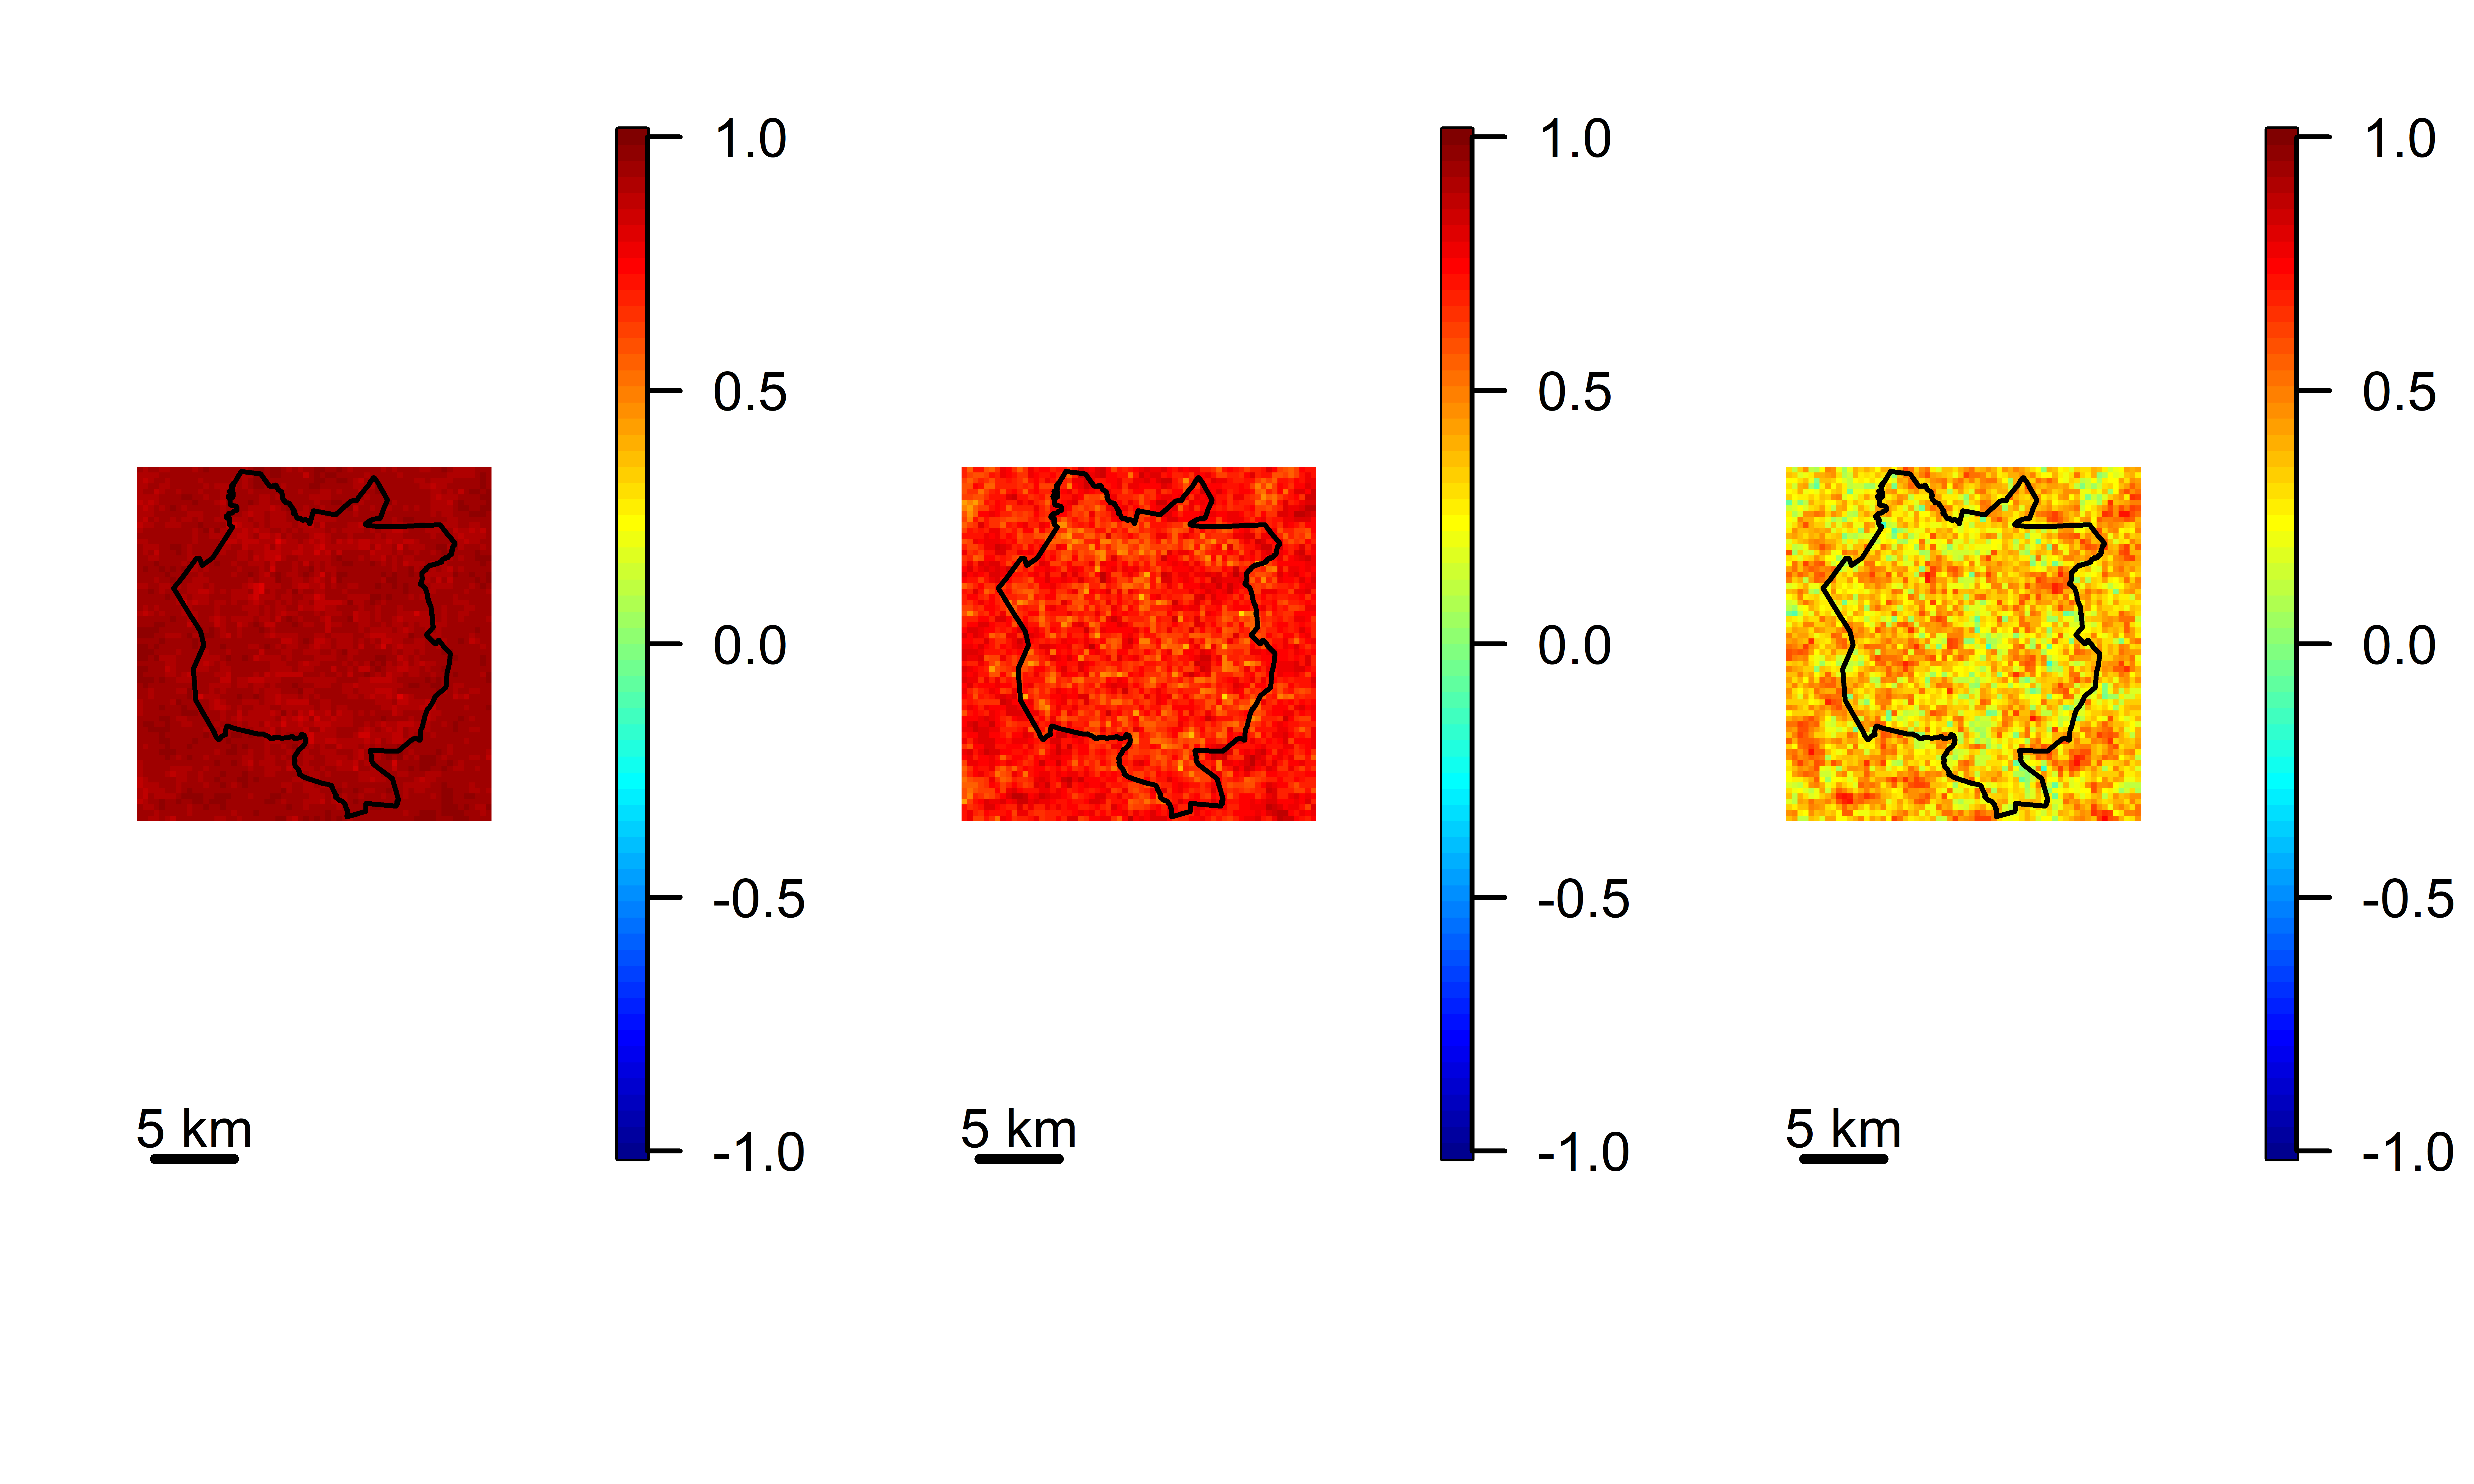
\includegraphics[width = \linewidth, height = 80mm]{Autocorrelations in the Latent Field - Major 0.png}
        \end{center}
       \FigureCaption{Autocorrelations in the latent field at different lags for clade 0 cases}
    \end{figure}

    \begin{figure}[H]
        \begin{center}
            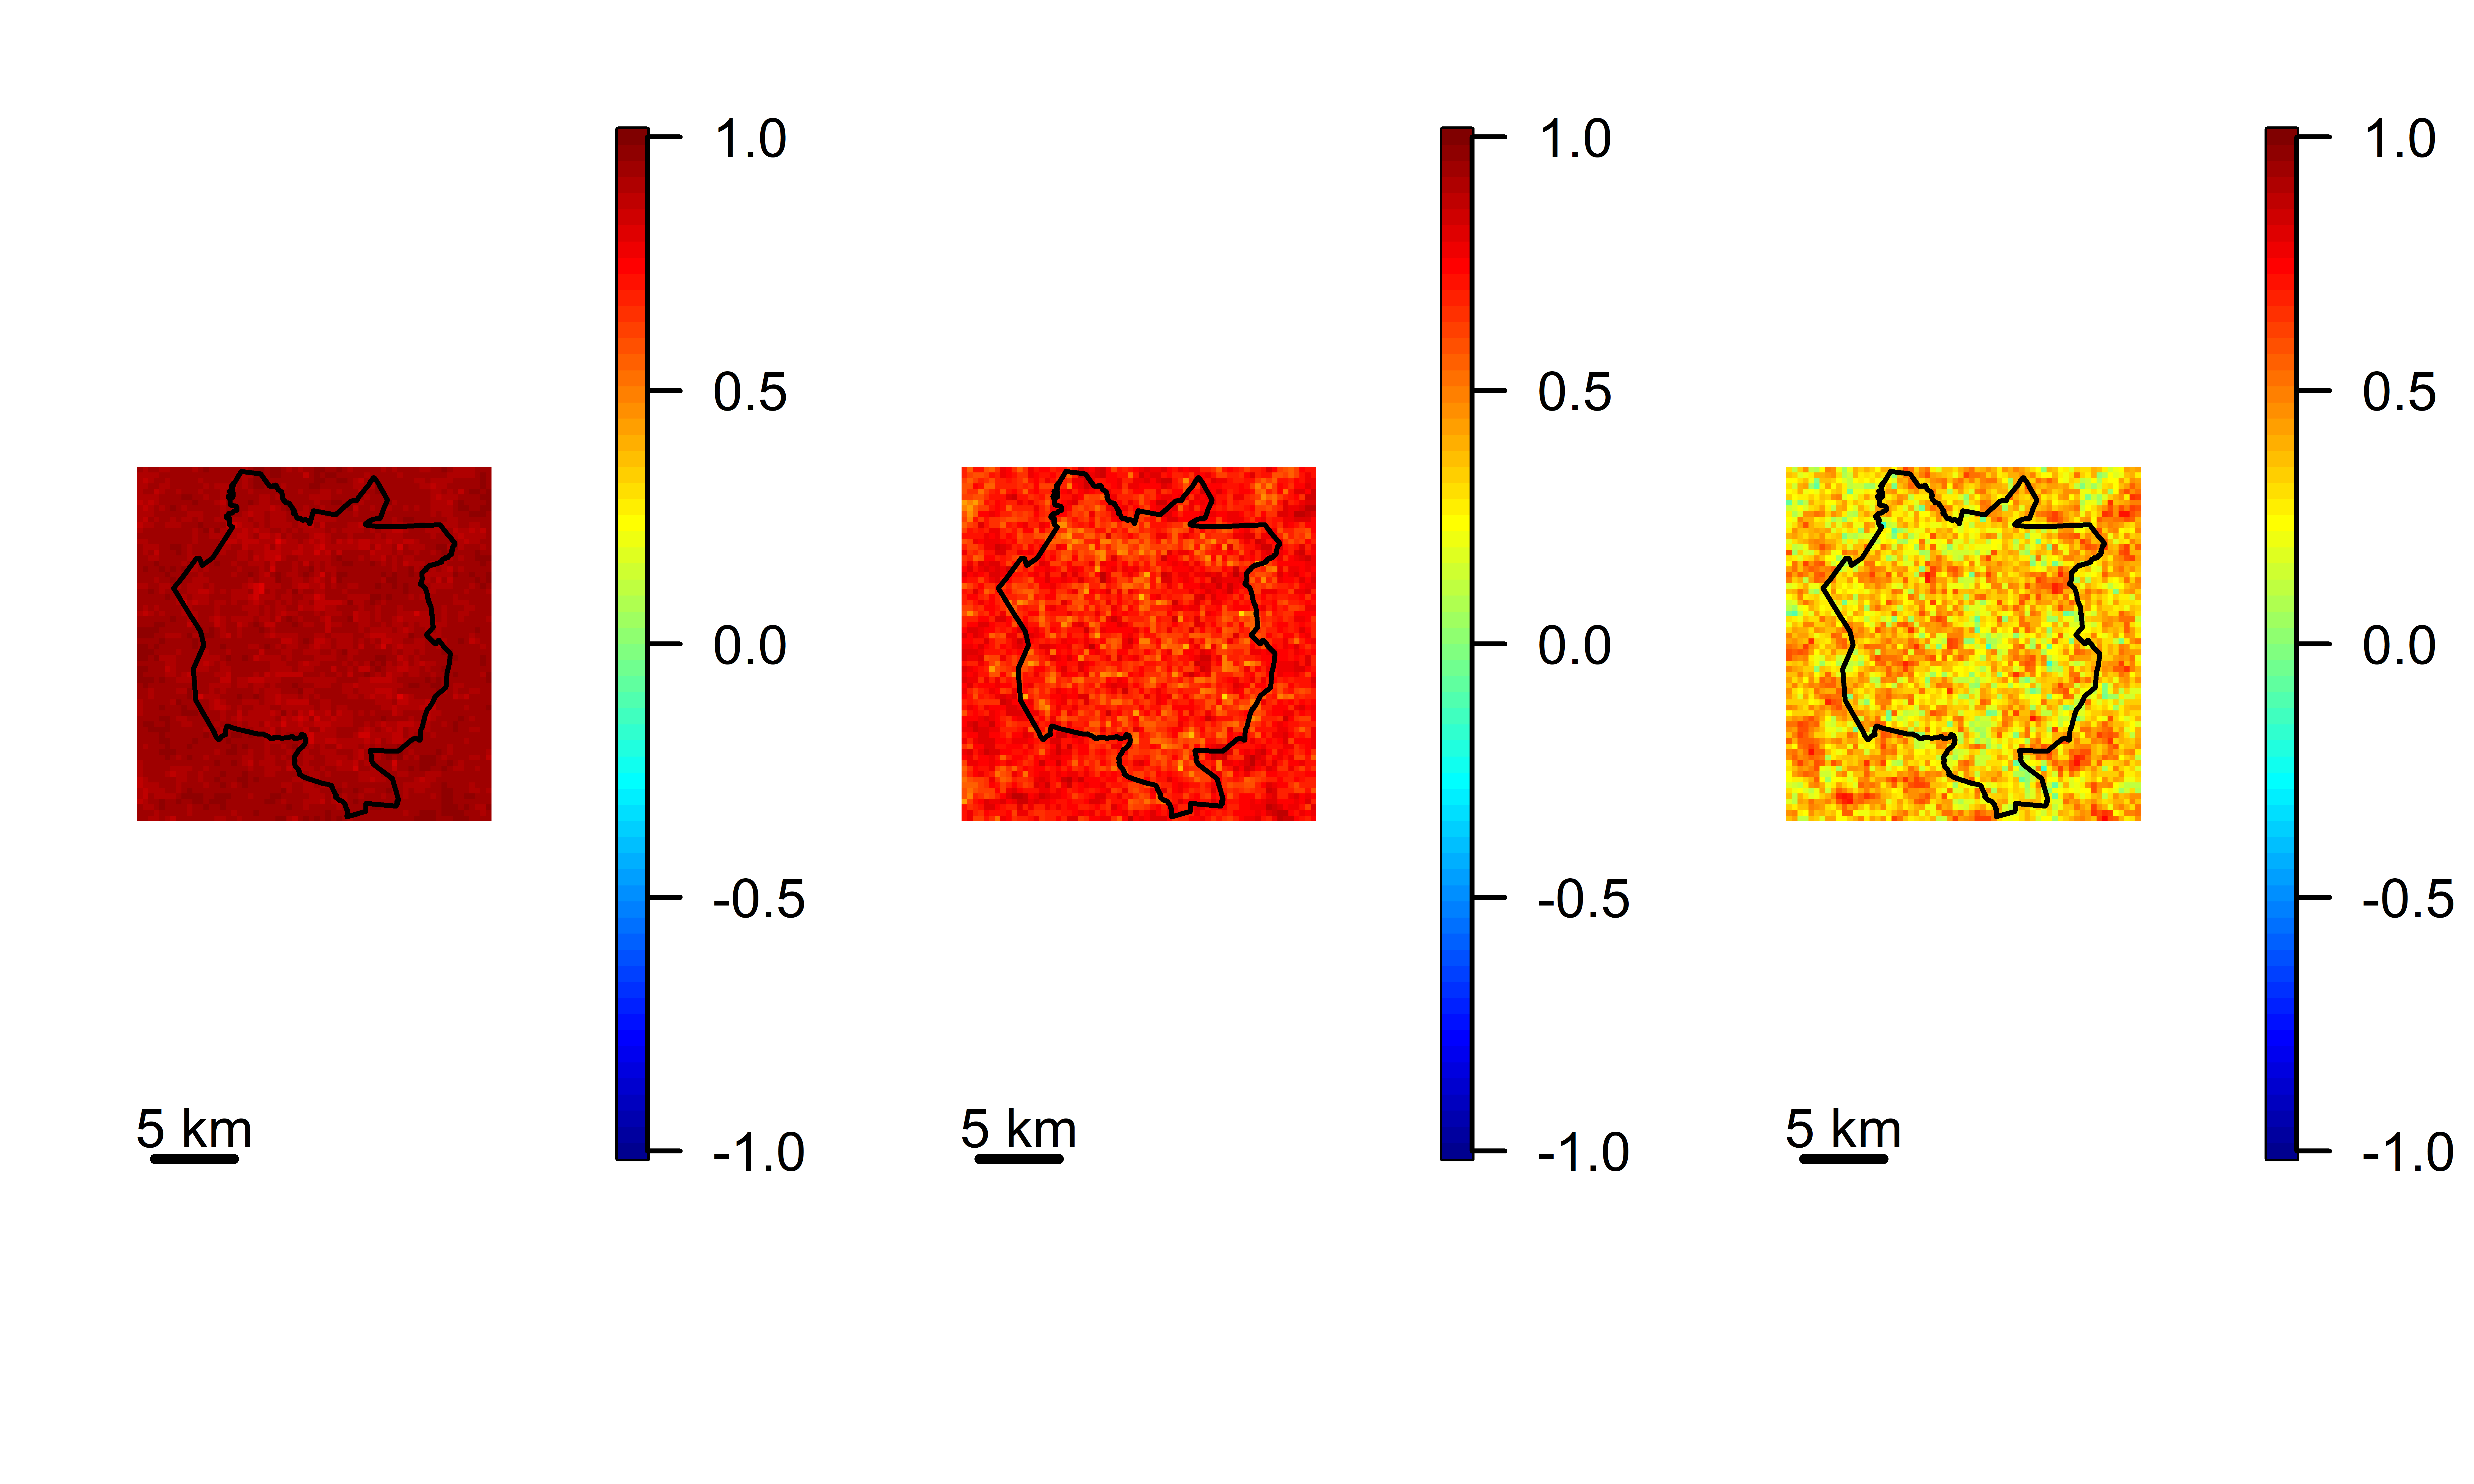
\includegraphics[width = \linewidth, height = 80mm]{Autocorrelations in the Latent Field - Major 2.png}
        \end{center}
        \FigureCaption{Autocorrelations in the latent field at different lags for clade 2 cases}
    \end{figure}

    \begin{figure}[H]
        \begin{center}
            \includegraphics[width = \linewidth, height = 80mm]{Autocorrelations in the Latent Field - Major 13456.png}
        \end{center}
        \FigureCaption{Autocorrelations in the latent field at different lags for the grouped clades}
    \end{figure}

    \begin{figure}[h]
        \begin{center}
            \includegraphics{Autocorrelation in the latent field - Multi-type.png}
        \end{center}
        \FigureCaption{Left to right: autocorrelations in the Gaussian latent field at lag 1, lag 5 and lag 15 for multi-type spatial model}
    \end{figure}

    \newpage
    \clearpage
    
\section*{Appendix 4: Autocorrelation of Parameters from the Point Process} \label{app:point-process}

    This subsection presents plots for the autocorrelation of parameters at different lags for the remaining spatio-temporal LGCP models and the multi-type LGCP model.

    \begin{figure}[h]
        \begin{center}
            \includegraphics[width = \linewidth, height = 80mm]{Autocorrelation plots of beta and eta - Major 0.png}
        \end{center}
        \FigureCaption{Autocorrelations in the latent field at different lags for spatio-temporal model with clade 0 cases}
    \end{figure}

    \begin{figure}[H]
        \begin{center}
            \includegraphics[width = \linewidth, height = 80mm]{Autocorrelation plots of beta and eta - Major 2.png}
        \end{center}
        \FigureCaption{Autocorrelations in the latent field at different lags for spatio-temporal model with clade 2 cases}
    \end{figure}

    \begin{figure}[H]
        \begin{center}
            \includegraphics[width = \linewidth, height = 80mm]{Autocorrelation plots of beta and eta - Major 13456.png}
        \end{center}
        \FigureCaption{Autocorrelation plots of the parameters of the latent field for the grouped clades}
    \end{figure}

\newpage

\section*{Appendix 5: Posterior Covariance Function} \label{app:covariance-function}

    This subsection presents posterior covariance function plots for the remaining spatio-temporal LGCP models and the multi-type LGCP model.

    \begin{figure}[H]
        \begin{center}
            \includegraphics[width=\linewidth]{Posterior Covariance Function - Major 2.png}
        \end{center}
        \FigureCaption{Plots of the posterior spatial covariance (Left) and temporal correlation (Right) for the Gaussian process of the spatio-temporal model for clade 2 cases}
    \end{figure}

    \begin{figure}[H]
        \begin{center}
            \includegraphics[width=\linewidth]{Posterior Covariance Function - Major 13456.png}
        \end{center}
        \FigureCaption{Plots of the posterior spatial covariance (Left) and temporal correlation (Right) for the spatio-temporal model for the grouped clades}
    \end{figure}

    \newpage


\section*{Appendix 6: Incidence Rates} \label{app:incidence-rates}

    This subsection presents plots of incidence rates for the remaining spatio-temporal LGCP models.

    \begin{figure}[H]
        \begin{center}
            \includegraphics[width=\linewidth]{Relative Risk Plot - SP - All Cases.png}
        \end{center}
        \FigureCaption{Incidence rate plot for the spatio-temporal model for all cases at every time point}
    \end{figure}

    \begin{figure}[H]
        \begin{center}
            \includegraphics[width=\linewidth]{Relative Risk Plot - SP - Major 0.png}
        \end{center}
        \FigureCaption{Incidence rate plot for the spatio-temporal model for clade 0 sub-lineage at different time point(months)}
    \end{figure}

    \begin{figure}[H]
        \begin{center}
            \includegraphics[width=\linewidth]{Relative Risk Plot - SP - Major 2.png}
        \end{center}
        \FigureCaption{Incidence rate plot for the spatio-temporal model for clade 2 sub-lineage at different time point(months)}
    \end{figure}

    \begin{figure}[H]
        \begin{center}
            \includegraphics[width=\linewidth]{Relative Risk Plot - SP - Major 13456.png}
        \end{center}
        \FigureCaption{Incidence rate plot for the spatio-temporal model for the grouped clades at different time point(months)}
    \end{figure}

    \newpage


\section*{Appendix 7: Standard Error of the Incidence Rates}

    This subsection presents the standard error of the incidence rate plots for the remaining spatio-temporal LGCP models.

    \begin{figure}[H]
        \begin{center}
            \includegraphics[width=\linewidth]{Standard Errors Plot - SP - All Cases.png}
        \end{center}
        \FigureCaption{Standard error plot of the incidence rate for the spatio-temporal model for all cases at every time point(months)}
    \end{figure}

    \begin{figure}[H]
        \begin{center}
            \includegraphics[width=\linewidth]{Standard Errors Plot - SP - Major 0.png}
        \end{center}
        \FigureCaption{Standard error plot of the incidence rate for the spatio-temporal model for clade 0 at different time point (months)}
    \end{figure}

    \begin{figure}[H]
        \begin{center}
            \includegraphics[width=\linewidth]{Standard Errors Plot - SP - Major 2.png}
        \end{center}
        \FigureCaption{Standard error plot of the incidence rate for the spatio-temporal model for clade 2 at different time point (months)}
    \end{figure}

    \begin{figure}[H]
        \begin{center}
            \includegraphics[width=\linewidth]{Standard Errors Plot - SP - Major 13456.png}
        \end{center}
        \FigureCaption{Standard error plot of the incidence rate for the spatio-temporal model for the grouped clades at different time point (months)}
    \end{figure}

    \newpage


\section*{Appendix 8: Prior and Posterior Density Plot} \label{app:density-plot}

    This subsection presents prior and posterior density plots for the remaining spatio-temporal LGCP models.

    \begin{figure}[H]
        \begin{center}
            \includegraphics[width = \linewidth, height = 80mm]{Prior and posterior density plots - All Cases.png}
        \end{center}
        \FigureCaption{Prior (continuous curve) and posterior (histogram) distribution for the parameters of the spatio-temporal LGCP model with all cases}
    \end{figure}

    \begin{figure}[H]
        \begin{center}
            \includegraphics[width = \linewidth, height = 80mm]{Prior and posterior density plots - Major 0.png}
        \end{center}
        \FigureCaption{Prior and posterior density plots for the spatio-temporal model for clade 0 cases}
    \end{figure}

    \begin{figure}[H]
        \begin{center}
            \includegraphics[width = \linewidth, height = 80mm]{Prior and posterior density plots - Major 2.png}
        \end{center}
        \FigureCaption{Prior and posterior density plots for the spatio-temporal model for clade 2 cases}
    \end{figure}

    \begin{figure}[H]
        \begin{center}
            \includegraphics[width = \linewidth, height = 80mm]{Prior and posterior density plots - Major 13456.png}
        \end{center}
        \FigureCaption{Prior and posterior density plots for the spatio-temporal model for the grouped clades}
    \end{figure}

    \newpage


\section*{Appendix 9: Inhomogeneous K Function} \label{app:inhomogeneous-k-function}

    This subsection presents Inhomogeneous K function plots for the remaining spatio-temporal LGCP models and the multi-type LGCP model.

    \begin{figure}[H]
        \begin{center}
            \includegraphics[width=\linewidth]{Inhomogeneous K Function - Major 2.png}
        \end{center}
        \FigureCaption{Inhomogeneous K Function for clade 2 cases}
    \end{figure}

    \begin{figure}[H]
        \begin{center}
            \includegraphics[width=\linewidth]{Inhomogeneous K Function - Major 13456.png}
        \end{center}
        \FigureCaption{Inhomogeneous K Function for the grouped clades}
    \end{figure}

    \newpage

\section*{Appendix 10: R Scripts}

The R codes are too long to be included in this document. They can be accessed on GitHub using this link \textit{https://github.com/donkalonga/MSc-Project-spatio-temporal-modelling} or by clicking \href{https://github.com/donkalonga/MSc-Project-spatio-temporal-modelling}{here}.

%\end{appendices}
